\documentclass{jhwhw}

\title{Tutorial A1\\Equations and Inequalities}
\author{Eytan Chong}
\date{2024-02-20}

\begin{document}
    \problem{}
        Determine whether each of the following systems of equations has a unique solution, infinitely many solutions, or no solutions. Find the solutions, where appropriate.

        \begin{enumerate}
            \item $\begin{cases}
                \begin{aligned}
                    a + 2b - 3c &= -5\\
                    -2a - 4b - 6c &= 10\\
                    3a + 7b - 2c &= -13
                \end{aligned}
            \end{cases}$
            \item $\begin{cases}
                \begin{aligned}
                x - y + 3z &= 3\\
                4x - 8y + 32z &= 24\\
                2x - 3y + 11z &= 4
                \end{aligned}
            \end{cases}$
            \item $\begin{cases}
                \begin{aligned}
                    x_1 + x_2 &= 5\\
                    2x_1 + x_2 + x_3 &= 13\\
                    4x_1 + 3x_2 + x_3 &= 23\\
                \end{aligned}
            \end{cases}$
            \item $\begin{cases}
                \begin{aligned}
                    \frac1p + \frac1q + \frac1r &= 5\\
                    \frac2p - \frac3q - \frac4r &= -11\\
                    \frac3p + \frac2q - \frac1r &= -6\\
                \end{aligned}
            \end{cases}$
            \item $\begin{cases}
                \begin{aligned}
                    2\sin\alpha - \cos\beta + 3\tan\gamma &= 3\\
                    4\sin\alpha + 2\cos\beta - 2\tan\gamma &= 2\\
                    6\sin\alpha - 3\cos\beta + \tan\gamma &= 9\\
                \end{aligned}
            \end{cases}$, where $0 \leq \alpha \leq 2\pi$, $0 \leq \beta \leq 2\pi$, and $0 \leq \gamma < \pi$.
        \end{enumerate}
    
    \solution
        \part          
            \boxt{
                Unique solution: $a = -9$, $b = 2$, $c = 0$
            }

        \part
            \boxt{
                No solution.
            }

        \part
            \boxt{
                Infinitely many solutions: $x_1 = 8-t$, $x_2 = t-3$, $x_3 = t$
            }

        \part
            \begin{center}
                $\dfrac1p = 2$, $\dfrac1q = -3$, $\dfrac1r = 6$
            \end{center}

            \boxt{
                Unique solution: $p = \dfrac12$, $q = -\dfrac13$, $r = \dfrac16$
            }

        \part
            \begin{center}
                $\sin\alpha = 1$, $\cos\beta = -1$, $\tan\gamma = 0$
            \end{center}

            \boxt{
                Unique solution: $\alpha = \dfrac\pi2$, $\beta = \pi$, $\gamma = 0$
            }
    
    \problem{}
        The following figure shows the circular cross section of a uniform log floating in a canal.

        \begin{center}
            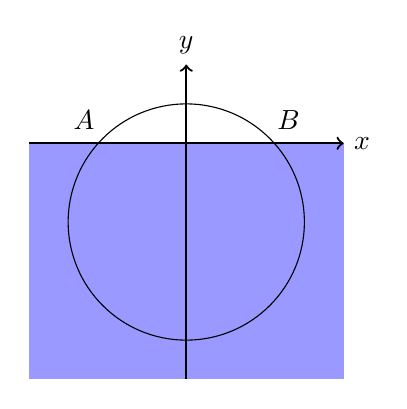
\begin{tikzpicture}
                \fill[blue!40!white] (0,0) rectangle (4,3);
                \draw (2,2) circle (1.5cm);
                \draw[thick,->] (0,3) -- (4,3) node[anchor=west] {$x$};
                \draw[thick,->] (2,0) -- (2,4) node[anchor=south] {$y$};
                \node[align=left] at (0.7, 3.3) {$A$};
                \node[align=left] at (3.3, 3.3) {$B$};
            \end{tikzpicture}
        \end{center}
        
        With respect to the axes shown, the circular outline of the log can be modelled by the equation 
        
        \begin{equation}\label{E::P2}
            x^2 + y^2 + ax + by + c = 0
        \end{equation}
        
        $A$ and $B$ are points on the outline that lie on the water surface. Given that the highest point of the log is 1-cm above the water surface when $AB$ is 40 cm apart horizontally, determine the values of $a$, $b$ and $c$ by forming a system of linear equations.

    \solution
        Since $AB = 40$, we have $A(-20, 0)$ and $B(20, 0)$. We also know $(0, 10)$ lies on the circle. Substituting these points into Equation~\ref{E::P2},

        \begin{equation*}
            \begin{cases}
                \begin{aligned}
                    -20a + c &= -400\\
                    20a + c &= -400\\
                    10b + c &= -100\\
                \end{aligned}
            \end{cases}
        \end{equation*}

        Solving the system of equations,

        \boxt{
            $a = 0$, $b = 30$, $c = -400$
        }

    \problem{}
        Find the exact solution set of the following inequalities.

        \begin{enumerate}
            \item $x^2 - 2 \geq 0$
            \item $4x^2 - 12x + 10 > 0$
            \item $x^2 + 4x + 13 < 0$
            \item $x^3 < 6x - x^2$
            \item $x^2(x-1)(x+3) \geq 0$
        \end{enumerate}

    \solution 
        \part 
            \begin{alignat*}{2}
                &&x^2 - 2 &\geq 0 \\
                \implies&& x^2 &\geq 2 \\
                \implies&& x &\leq -\sqrt2 \lor x \geq \sqrt2
            \end{alignat*}

            \boxt{
                Solution set: $\left\{ x \in \mathbb{R}\colon x \leq -\sqrt2 \lor x \geq \sqrt2 \right\}$
            }

        \part
            \begin{alignat*}{2}
                &&4x^2-12x+10&>0\\
                \implies&& x^2-3x+\frac52 &> 0 \\
                \implies&& x^2-3x+\left(\frac32\right)^2 - \left(\frac32\right)^2 + \frac52 &> 0\\
                \implies&& \left(x-\frac32\right)^2+\frac{19}4 &> 0
            \end{alignat*}

            Since $\left(x-\dfrac32\right)^2 \geq 0$, all $x \in \mathbb{R}$ satisfy the inequality.

            \boxt{
                Solution set: $\mathbb{R}$
            }

        \part
            \begin{alignat*}{2}
                &&x^2 + 4x + 13 < 0\\
                \implies&& x^2 + 4x + 4 + 9 < 0\\
                \implies&& (x+2)^2 + 9 < 0
            \end{alignat*}

            Since $(x+2)^2 \geq 0$, there is no solution to the inequality.

            \boxt{
                Solution set: $\varnothing$
            }

        \part 
            \begin{alignat*}{2}
                &&x^3 < 6x-x^2\\
                \implies&& x(x+3)(x-2) < 0\\
            \end{alignat*}

            \begin{center}
                \begin{tikzpicture}
                    \draw[-latex] (-5,0) -- (4,0) node[right]{$x$};
                    \foreach \x in  {-3, 0, 2}
                    \draw[shift={(\x,0)}] (0pt,3pt) -- (0pt,-3pt);
                    \foreach \x in {-3, 0, 2}
                    \draw[shift={(\x,-3pt)}] node[below] 
                    {$\x$};
                    \draw[very thick, -o, color=red] (-5, 0) -- (-2.9, 0);
                    \draw[very thick, o-o, color=red] (-0.1, 0) -- (2.1, 0);
                    \node[anchor=south, align=center] at (-4, 0) {$-$};
                    \node[anchor=south, align=center] at (-1.5, 0) {$+$};
                    \node[anchor=south, align=center] at (1, 0) {$-$};
                    \node[anchor=south, align=center] at (3, 0) {$+$};
                \end{tikzpicture}
            \end{center}

            \begin{equation*}
                \implies x < -3 \lor 0 < x < 2
            \end{equation*}

            \boxt{
                Solution set: $\{x \in \mathbb{R} \colon x < -3 \lor 0 < x < 2\}$
            }

        \part

            \begin{equation*}
                x^2(x-1)(x+3) \geq 0
            \end{equation*}

            \begin{center}
                \begin{tikzpicture}
                    \draw[-latex] (-5,0) -- (3,0) node[right]{$x$};
                    \foreach \x in  {-3, 0, 1}
                    \draw[shift={(\x,0)}] (0pt,3pt) -- (0pt,-3pt);
                    \foreach \x in {-3, 0, 1}
                    \draw[shift={(\x,-3pt)}] node[below] 
                    {$\x$};
                    \draw[very thick, -*, color=red] (-5, 0) -- (-2.9, 0);
                    \draw[very thick, *-, color=red] (0.9, 0) -- (2.9, 0);
                    \path [draw=red, fill=red] (0,0) circle (3pt);

                    \node[anchor=south, align=center] at (-4, 0) {$+$};
                    \node[anchor=south, align=center] at (-1.5, 0) {$-$};
                    \node[anchor=south, align=center] at (0.5, 0) {$-$};
                    \node[anchor=south, align=center] at (2, 0) {$+$};
                \end{tikzpicture}
            \end{center}

            \begin{equation*}
                \implies x \leq -3 \lor x = 0 \lor x \geq 1
            \end{equation*}

            \boxt{
                Solution set: $\{x \in \mathbb{R} \colon x \leq -3 \lor x = 0 \lor x \geq 1\}$
            }

    \problem{}
        Find the exact solution set of the following inequalities.

        \begin{enumerate}
            \item $\abs{3x+5} < 4$
            \item $\abs{x-2} < 2x$
        \end{enumerate}

    \solution
        \part
            \begin{equation*}
                \abs{3x+5} < 4
            \end{equation*}

            \case{1}{$3x + 5 < 4$}
                \begin{alignat*}{2}
                    &&3x + 5 &< 4\\
                    \implies&& 3x &< -1\\
                    \implies&& x &< -\frac13
                \end{alignat*}

            \case{2}{$-(3x+5) < 4$}

                \begin{alignat*}{2}
                    &&-(3x+5) &< 4\\
                    \implies&& -3x - 5 &< 4\\
                    \implies&& -3x &< 9 \\
                    \implies&& x &> -3
                \end{alignat*}

            Combining both inequalities, we have $-3 < x < -\dfrac13$.
            
            \boxt{
                Solution set: $\left\{x \in \mathbb{R} \colon -3 < x< -\dfrac13\right\}$
            }

        \part
            \case{1}{$x-2 < 2x$}
                \begin{alignat*}{2}
                    &&x - 2 &< 2x \\
                    \implies&& x &> -2
                \end{alignat*}

            \case{2}{$-(x-2) < 2x$}
                \begin{alignat*}{2}
                    &&-(x-2) &< 2x \\
                    \implies&& -x + 2 &< 2x\\
                    \implies&& 3x &> 2\\
                    \implies&& x &> \dfrac23
                \end{alignat*}

            Combining both inequalities, we have $x > \dfrac23$.

            \boxt{
                Solution set: $\left\{x \in \mathbb{R} \colon x > \dfrac23\right\}$
            }

    \problem{}
        It is given that $p(x) = x^4 + ax^3 + bx^2 + cx + d$, where $a$, $b$, $c$ and $d$ are constants. Given that the curve with equation $y = p(x)$ is symmetrical about the $y$-axis, and that it passes through the points with coordinates $(1,2)$ and $(2,11)$, find the values of $a$, $b$, $c$ and $d$.

    \solution
        We know that $(1,2)$ and $(2,11)$ lie on the curve. Since $y = p(x)$ is symmetrical about the $y$-axis, we have that $(-1,2)$ and $(-2,11)$ also lie on the curve. Substituting these points into $y = p(x)$, we obtain the following system of equations.

        \begin{equation*}
            \begin{cases}
                \begin{aligned}
                    a+b+c+d &= 1\\
                    a-b+c-d &= -1\\
                    8a+4b+2c+d &= -5\\
                    8a-4b+2c-d &= 5\\
                \end{aligned}
            \end{cases}
        \end{equation*}

        Solving the system of equations,

        \boxt{
            $a = 0$, $b = -2$, $c = 0$, $d=3$
        }
        

    \problem{}
        Mr Mok invested \$50,000 in three funds A, B and C. Each fund has a different risk level and offers a different rate of return.

        In 2016, the rates of return for funds A, B and C were 6\%, 8\%, and 10\% respectively and Mr Mok attained a total return of \$3,700. He invested twice as much money in Fund A as in Fund C. How much did he invest in each of the funds in 2016?

    \solution
        Let $a$, $b$ and $c$ be the amount of money Mr Mok invested in Funds A, B and C respectively, in dollars. We thus have the following system of equations.

        \begin{equation*}
            \begin{cases}
                \begin{aligned}
                    a+b+c &= 50000\\
                    \dfrac{6}{100}a + \dfrac{8}{100}b + \dfrac{10}{100}c &= 3700\\
                    a &= 2c
                \end{aligned}
            \end{cases}
        \end{equation*}

        Solving the system of equations, we have $a = 30000$, $b = 5000$ and $c = 15000$.

        \boxt{
            Mr Mok invested \$30,000, \$5,000 and \$15,000 in Funds A, B and C respectively.
        }

    \problem{}
        Solve the following inequalities with exact answers.

        \begin{enumerate}
            \item $2x-1 \geq \dfrac6x$
            \item $x-\dfrac1x < 1$
            \item $-1 < \dfrac{2x+3}{x-1} < 1$
        \end{enumerate}

    \solution
        \part
             \begin{alignat*}{2}
                &&2x-1 &\geq \dfrac6x, \qquad x \neq 0 \\
                \implies&& x^2(2x-1) &\geq 6x\\
                \implies&& x^2(2x-1) - 6x &\geq 0\\
                \implies&& x(x(2x-1) - 6) &\geq 0\\
                \implies&& x\left(2x^2-x-6\right) &\geq 0\\
                \implies&& x(2x+3)(x-2) &\geq 0
             \end{alignat*}

             \begin{center}
                \begin{tikzpicture}
                    \draw[-latex] (-2.5,0) -- (3,0) node[right]{$x$};
                    \foreach \x in  {-1.5, 0, 2}
                    \draw[shift={(\x,0)}] (0pt,3pt) -- (0pt,-3pt);
                    \foreach \x in {-1.5, 0, 2}
                    \draw[shift={(\x,-3pt)}] node[below] 
                    {$\x$};

                    \draw[very thick, *-o, color=red] (-1.6, 0) -- (0.12, 0);
                    \draw[very thick, *-, color=red] (1.9, 0) -- (2.9, 0);

                    \node[anchor=south, align=center] at (-2, 0) {$-$};
                    \node[anchor=south, align=center] at (-0.75, 0) {$+$};
                    \node[anchor=south, align=center] at (1, 0) {$-$};
                    \node[anchor=south, align=center] at (2.5, 0) {$+$};
                \end{tikzpicture}
            \end{center}

            \boxt{
                $-\dfrac32 \leq x < 0 \lor x \geq 2$
            }

        \part
            \begin{alignat*}{2}
                &&x - \dfrac1x &< 1, \qquad x \neq 0 \\
                \implies&&x^3 - x &< x^2\\
                \implies&&x^3 - x^2 - x &< 0\\
                \implies&&x\left(x^2 - x - 1\right) &< 0\\
                \implies&&x(x-\phi)(x-\bar{\phi}) &< 0\\
            \end{alignat*}

            \begin{center}
                \begin{tikzpicture}
                    \draw[-latex] (-1.618,0) -- (2.618,0) node[right]{$x$};
                    \foreach \x in  {-0.618, 0, 1.618}
                    \draw[shift={(\x,0)}] (0pt,3pt) -- (0pt,-3pt);

                    \draw[shift={(-0.618,-3pt)}] node[below] 
                    {$\bar{\phi}$};
                    \draw[shift={(0,-3pt)}] node[below] 
                    {0};
                    \draw[shift={(1.618,-3pt)}] node[below] 
                    {$\phi$};

                    \draw[very thick, -*, color=red] (-1.618, 0) -- (-0.518, 0);
                    \draw[very thick, o-*, color=red] (-0.12, 0) -- (1.718, 0);

                    \node[anchor=south, align=center] at (-1.118, 0) {$-$};
                    \node[anchor=south, align=center] at (-0.309, 0) {$+$};
                    \node[anchor=south, align=center] at (0.809, 0) {$-$};
                    \node[anchor=south, align=center] at (2.118, 0) {$+$};
                \end{tikzpicture}
            \end{center}

            \boxt{
                $x \leq \bar{\phi} \lor 0 < x \leq \phi$
            }

        \part
            \begin{alignat*}{2}
                && -1 &< \dfrac{2x+3}{x-1} < 1 \\
                \implies&& -1 &< \dfrac{(2x-2)+5}{x-1} < 1 \\
                \implies&& -1 &< 2 + \dfrac5{x-1} < 1\\
                \implies&& -3 &< \dfrac5{x-1} < -1\\
                \implies&& -\dfrac35 &< \dfrac1{x-1} < -\dfrac15\\
                \implies&& -5 &< x-1 < -\dfrac53\\
                \implies&& -4 &< x < -\dfrac23
            \end{alignat*}
            
            \boxt{
                $-4 < x < -\dfrac23$
            }
    
    \problem{}
        Without using a calculator, solve the inequality $\dfrac{x^2+x+1}{x^2+x-2} < 0$.

    \solution
        Observe that

            \begin{equation*}
                \begin{aligned}
                    x^2 + x + 1 &= x^2 + x + \left(\dfrac12\right)^2 - \left(\dfrac12\right)^2 + 1 \\
                    &= \left(x + \dfrac12\right)^2 + \dfrac34 \\
                    &> 0
                \end{aligned}
            \end{equation*}

        Thus, the inequality reduces to $\dfrac1{x^2+x-2} < 0$

        \begin{alignat*}{2}
            &&\dfrac1{x^2+x-2} &< 0 \\
            \implies&& x^2 + x - 1 &< 0\\
            \implies&& (x-1)(x+2) &< 0\\
        \end{alignat*}

        
        \begin{center}
            \begin{tikzpicture}
                \draw[-latex] (-3,0) -- (2,0) node[right]{$x$};
                \foreach \x in  {-2, 1}
                \draw[shift={(\x,0)}] (0pt,3pt) -- (0pt,-3pt);

                \foreach \x in  {-2, 1}
                \draw[shift={(\x,-3pt)}] node[below] 
                {$\x$};

                \draw[very thick, o-o, color=red] (-2.12, 0) -- (1.12, 0);

                \node[anchor=south, align=center] at (-2.5, 0) {$+$};
                \node[anchor=south, align=center] at (-0.5, 0) {$-$};
                \node[anchor=south, align=center] at (1.5, 0) {$+$};
            \end{tikzpicture}
        \end{center}

        \boxt{
            $-2 < x < 1$
        }

    \problem{}
        Solve the following inequalities using a graphical method.

        \begin{enumerate}
            \item $\abs{3x+1} < (4x+3)^2$
            \item $\abs{3x+1} \geq \abs{2x+7}$
            \item $\abs{x-2} \geq x + \abs{x}$
            \item $5x^2 + 4x - 3 > \ln{(x+1)}$
        \end{enumerate}

    \solution
        \part
            \begin{center}
                \begin{tikzpicture}[trim axis left, trim axis right]
                    \begin{axis}[
                        domain = -2.5:0.5,
                        samples = 50,
                        axis y line=middle,
                        axis x line=middle,
                        xlabel = {$x$},
                        ylabel = {$y$},
                        ymax=10,
                        legend cell align={left},
                        legend pos=outer north east,
                        after end axis/.code={
                            \path (axis cs:0,0) 
                                node [anchor=north] {$O$};
                            }
                        ]
                        \addplot[red!50, name path=f1] {abs(3*x+1)};

                        \addlegendentry{$y=\abs{3x+1}$};

                        \addplot[blue!50, name path=f2] {(4*x+3)^2};

                        \addlegendentry{$y=(4x+3)^2$};

                        \fill [name intersections={of=f1 and f2,by={E1,E2}}] (E1) circle[radius=2.5pt] node[anchor=south east] {$(-1.14, 2.42)$};
                        
                        \fill (E2) circle[radius=2.5pt] node[anchor=south east] {$(-0.549, 0.647)$};
                    \end{axis}
                \end{tikzpicture}
            \end{center}

            \boxt{
                $x < -1.14 \lor x > -0.549$
            }

        \part
            \begin{center}
                \begin{tikzpicture}[trim axis left, trim axis right]
                    \begin{axis}[
                        domain = -6:8,
                        samples = 50,
                        axis y line=middle,
                        axis x line=middle,
                        xlabel = {$x$},
                        ylabel = {$y$},
                        ymax=20,
                        legend cell align={left},
                        legend pos=outer north east,
                        after end axis/.code={
                            \path (axis cs:0,0) 
                                node [anchor=north] {$O$};
                            }
                        ]
                        \addplot[red!50, name path=f1] {abs(3*x+1)};

                        \addlegendentry{$y=\abs{3x+1}$};

                        \addplot[blue!50, name path=f2] {abs(2*x + 7)};

                        \addlegendentry{$y=\abs{2x+7}$};

                        \fill [name intersections={of=f1 and f2,by={E1,E2}}] (E1) circle[radius=2.5pt] node[anchor=east] {$(-1.6, 3.8)$};
                        
                        \fill (E2) circle[radius=2.5pt] node[anchor=east] {$(6, 19)$};
                    \end{axis}
                \end{tikzpicture}
            \end{center}

            \boxt{
                $x \leq -1.6 \lor x \geq 6$
            }

        \part
            \begin{center}
                \begin{tikzpicture}[trim axis left, trim axis right]
                    \begin{axis}[
                        domain = -2:3,
                        samples = 50,
                        axis y line=middle,
                        axis x line=middle,
                        xlabel = {$x$},
                        ylabel = {$y$},
                        ymax=5,
                        legend cell align={left},
                        legend pos=outer north east,
                        after end axis/.code={
                            \path (axis cs:0,0) 
                                node [anchor=north] {$O$};
                            }
                        ]
                        \addplot[red!50, name path=f1] {abs(x-2)};

                        \addlegendentry{$y=\abs{x-2}$};

                        \addplot[blue!50, name path=f2] {x + abs(x)};

                        \addlegendentry{$y=x+\abs{x}$};

                        \fill [name intersections={of=f1 and f2,by={E1}}] (E1) circle[radius=2.5pt] node[anchor=west] {$(0.667, 1.33)$};
                    \end{axis}
                \end{tikzpicture}
            \end{center}

            \boxt{
                $x \leq 0.667$  
            }

        \part
            \begin{center}
                \begin{tikzpicture}[trim axis left, trim axis right]
                    \begin{axis}[
                        domain = -2:3,
                        samples = 50,
                        axis y line=middle,
                        axis x line=middle,
                        xlabel = {$x$},
                        ylabel = {$y$},
                        ymax=5,
                        legend cell align={left},
                        legend pos=outer north east,
                        after end axis/.code={
                            \path (axis cs:0,0) 
                                node [anchor=north] {$O$};
                            }
                        ]
                        \addplot[red!50, name path=f1] {5*x^2 + 4*x -3};

                        \addlegendentry{$y=5x^2+4x-3$};

                        \addplot[blue!50, name path=f2] {ln(x+1)};

                        \addlegendentry{$y=\ln(x+1)$};

                        \fill [name intersections={of=f1 and f2,by={E1, E2}}] (E1) circle[radius=2.5pt] node[anchor=north west] {$(-0.916, -2.47)$};

                        \fill (E2) circle[radius=2.5pt] node[anchor=south west] {$(0.518, 0.418)$};

                        \addplot[mark=none, black, thick, dotted] coordinates {(-1, 5) (-1,-4)};

                        \addlegendentry{$x=-1$}
                    \end{axis}
                \end{tikzpicture}
            \end{center}

            \boxt{
                $-1 < x < -0.916 \lor x > 0.518$
            }

    \problem{}
        Sketch the graphs of $y = \abs{x-20}$ and $y=\dfrac1x$ on the same diagram. Hence or otherwise, solve the inequality $\abs{x-20} < \dfrac1x$, leaving your anwers correct to 2 decimal places.

    \solution
        \begin{center}
            \begin{tikzpicture}[trim axis left, trim axis right]
                \begin{axis}[
                    domain = -5:35,
                    samples = 81,
                    axis y line=middle,
                    axis x line=middle,
                    xlabel = {$x$},
                    ylabel = {$y$},
                    ymax=20,
                    ymin=-20,
                    legend cell align={left},
                    legend pos=outer north east,
                    xticklabels={20},
                    xtick={20},
                    after end axis/.code={
                        \path (axis cs:0,0) 
                            node [anchor=north east] {$O$};
                        }
                    ]
                    \addplot[red!50, name path=f1] {abs(x-20)};

                    \addlegendentry{$y = \abs{x-20}$};

                    \addplot[blue!50, name path=f2, unbounded coords=jump] {50 /x};

                    \addlegendentry{$y=x^{-1}$};

                    \fill [name intersections={of=f1 and f2,by={E1, E2, E3}}] (E1) circle[radius=2.5pt] node[anchor=north west] {$(0.05, 19.95)$};

                    \fill (E2) circle[radius=2.5pt] node[anchor=south east] {$(19.05, 0.05)$};

                    \fill (E3) circle[radius=2.5pt] node[anchor=south west] {$(20.05, 0.05)$};
                \end{axis}
            \end{tikzpicture}
        \end{center}

        \boxt{
            $0 < x < 0.05 \lor 19.95 < x < 20.05$
        }

    \problem{}
        Solve the inequality $\dfrac{x-9}{x^2-9} \leq 1$. Hence, solve the inequalities

        \begin{enumerate}
            \item $\dfrac{\abs{x}-9}{x^2-9} \leq 1$
            \item $\dfrac{x+9}{x^2-9} \geq -1$
        \end{enumerate}

    \solution
        \begin{alignat*}{2}
            &&\dfrac{x-9}{x^2-9} &\leq 1\\
            \implies&& (x-9)\left(x^2-9\right) &\leq \left(x^2 - 9\right)^2\\
            \implies&& x^3 - 9x^2 -9x +81 &\leq x^4 - 18x^2 + 81\\
            \implies&& x^4 - x^3 - 9x^2 + 9x &\geq 0\\
            \implies&& (x+3)x(x-1)(x-3) &\geq 0\\
        \end{alignat*}

        \begin{center}
            \begin{tikzpicture}
                \draw[-latex] (-4,0) -- (4,0) node[right]{$x$};
                \foreach \x in  {-3, 0, 1, 3}
                \draw[shift={(\x,0)}] (0pt,3pt) -- (0pt,-3pt);
                \foreach \x in  {-3, 0, 1, 3}
                \draw[shift={(\x,-3pt)}] node[below] 
                {$\x$};

                \draw[very thick, -o, color=red] (-4, 0) -- (-2.88, 0);
                \draw[very thick, *-*, color=red] (-0.12, 0) -- (1.12, 0);
                \draw[very thick, o-, color=red] (2.88, 0) -- (3.9, 0);


                \node[anchor=south, align=center] at (-3.5, 0) {$+$};
                \node[anchor=south, align=center] at (-1.5, 0) {$-$};
                \node[anchor=south, align=center] at (0.5, 0) {$+$};
                \node[anchor=south, align=center] at (3.5, 0) {$-$};
            \end{tikzpicture}
        \end{center}

        \boxt{
            $x < -3 \lor 0 \leq x \leq 1 \lor x > 3$
        }
        
        \part

        Consider the substitution $x \mapsto \abs{x}$ on the inequality $\dfrac{x-9}{x^2-9} \leq 1$. This yields our desired inequality $\dfrac{\abs{x}-9}{x^2-9} \leq 1$. Hence,

        \begin{equation*}
            \abs{x} < -3 \lor 0 \leq \abs{x} \leq 1 \lor \abs{x} > 3
        \end{equation*}

        \case{1}{$\abs{x} < -3$}\newline
            \indent No solution.

        \medskip
        \case{2}{$0 \leq \abs{x} \leq 1$}
            \begin{equation*}
                -1 \leq x \leq 1
            \end{equation*}

        \case{3}{$\abs{x} > 3$}
            \begin{equation*}
                x < -3 \lor x > 3
            \end{equation*}

        Combining all three cases, we finally have

        \boxt{
            $x < -3 \lor -1 \leq x \leq 1 \lor x > 3$
        }

        \part
            Consider the substitution $x \mapsto -x$ on the inequality $\dfrac{x-9}{x^2-9} \leq 1$. This yields $\dfrac{-x-9}{x^2-9} \leq 1$, which is equivalent to our desired inequality  $\dfrac{x+9}{x^2-9} \geq -1$. Hence, 

            \begin{equation*}
                -x < -3 \lor 0 \leq -x \leq 1 \lor -x > 3
            \end{equation*}

            \case{1}{$-x < -3$}
                \begin{equation*}
                    x > 3
                \end{equation*}
            
            \case{2}{$0 \leq -x \leq 1$}
                \begin{equation*}
                    -1 \leq x \leq 0
                \end{equation*}

            \case{3}{$-x > 3$}
                \begin{equation*}
                    x < -3
                \end{equation*}

            Combining all three cases, we finally have

            \boxt{
                $x < -3 \lor -1 \leq x \leq 0 \lor x > 3$
            }

    \problem{}
        Solve the inequality $\dfrac{x-5}{1-x} \geq 1$. Hence, solve $0 < \dfrac{1-\ln x}{\ln x -5} \leq 1$.

    \solution
        \begin{alignat*}{2}
            &&\dfrac{x-5}{1-x} &\geq 1, \qquad x \neq 1\\
            \implies&& (x-5)(1-x) &\geq \left(1-x\right)^2\\
            \implies&& 2x^2-8x+6 &\leq 0\\
            \implies&& 2(x-1)(x-3) &\leq 0\\
        \end{alignat*}

        \begin{center}
            \begin{tikzpicture}
                \draw[-latex] (0,0) -- (4,0) node[right]{$x$};
                \foreach \x in  {1, 3}
                \draw[shift={(\x,0)}] (0pt,3pt) -- (0pt,-3pt);
                \foreach \x in  {1, 3}
                \draw[shift={(\x,-3pt)}] node[below] 
                {$\x$};

                \draw[very thick, o-*, color=red] (0.88, 0) -- (3.12, 0);


                \node[anchor=south, align=center] at (0.5, 0) {$+$};
                \node[anchor=south, align=center] at (2, 0) {$-$};
                \node[anchor=south, align=center] at (3.5, 0) {$+$};
            \end{tikzpicture}
        \end{center}

        \boxt{
            $1 < x \leq 3$
        }

        Consider the substitution $x \mapsto \ln x$ on the inequality $\dfrac{x-5}{1-x} \geq 1$. This yields our desired inequality $0 < \dfrac{1-\ln x}{\ln x -5} \leq 1$. Hence, 

        \begin{alignat*}{2}
            &&1 < \ln x &\leq 3 \\
            \implies&& e < x &\leq e^3
        \end{alignat*}

        \boxt{
            $e < x \leq e^3$
        }

    \problem{}
        A small rocket is launched from a height of 72 m from the ground. The heigh of the rocket in metres, $h$, is represented by the equation $h = -16t^2 + 64t+72$, where $t$ is the time in seconds after the launch.

        \begin{enumerate}
            \item Sketch the graph of $h$ against $t$.
            \item Determine the number of seconds that the rocket will remain at or above 100 m from the ground.
        \end{enumerate}

    \solution
        \part
            \begin{center}
                \begin{tikzpicture}[trim axis left, trim axis right]
                    \begin{axis}[
                        domain = 0:5.5,
                        samples = 101,
                        axis y line=middle,
                        axis x line=middle,
                        xlabel = {$t$},
                        ylabel = {$h$},
                        xtick={4.92},
                        xticklabels={4.92},
                        ytick={136},
                        yticklabels={136},
                        ymax=165,
                        legend cell align={left},
                        legend pos=outer north east,
                        after end axis/.code={
                            \path (axis cs:0,0) 
                                node [anchor=north east] {$O$};
                            }
                        ]

                        \path [draw=red, fill=red] (axis cs:2, 136) circle (3pt) node[anchor=south west] {$(2, 136)$};


                        \addplot[red!50, domain=0:4.92] {-16*x^2 + 64*x + 72)};

                        \addlegendentry{$h = -16t^2 + 64t+72$};

                        \addplot[white!0]{165};
                    \end{axis}
                \end{tikzpicture}
            \end{center}

        \part
            \begin{alignat*}{2}
                &&h &\geq 100\\
                \implies&& -16t^2 + 64t+72 &\geq 100\\
                \implies&& -16t^2 + 64t-28 &\geq 0 \\
                \implies&& 16t^2 - 64t+28 &\geq 0 \\
                \implies&& 4(2t-1)(2t-7) &\leq 0\\
            \end{alignat*}

            \begin{center}
                \begin{tikzpicture}
                    \draw[-latex] (-0.5,0) -- (4.5,0) node[right]{$x$};
                    \foreach \x in  {0.5, 3.5}
                    \draw[shift={(\x,0)}] (0pt,3pt) -- (0pt,-3pt);
                    \foreach \x in  {0.5, 3.5}
                    \draw[shift={(\x,-3pt)}] node[below] 
                    {$\x$};
    
                    \draw[very thick, *-*, color=red] (0.38, 0) -- (3.65, 0);
    
    
                    \node[anchor=south, align=center] at (0, 0) {$+$};
                    \node[anchor=south, align=center] at (2,0) {$-$};
                    \node[anchor=south, align=center] at (4, 0) {$+$};
                \end{tikzpicture}
            \end{center}

            \boxt{
                The rocket will remain at or above 100 m from the ground for $\dfrac72-\dfrac12 = 3$ seconds.
            }
            

    \problem{}
        Xinxin, a new graduate, starts work at a company with an initial monthly pay of \$2,000. For every subsequent quarter that she works, she will get a pay increase of 5\%, leading to a new monthly pay of $2000(1.05)^{n-1}$ dollars in the $n$th quarter, where $n$ is a positive integer. She also gives a regular donation of \$$300n$ in the $n$th quarter that she works. However, she will stop the donation when her monthly pay falls below the donation amount. At which quarter will this first happen?

    \solution
        Consider the curves $y = 2000(1.05)^{x-1}$ and $y=300x$.

        \begin{center}
            \begin{tikzpicture}[trim axis left, trim axis right]
                \begin{axis}[
                    domain = 0:13,
                    samples = 81,
                    axis y line=middle,
                    axis x line=middle,
                    xlabel = {$x$},
                    ylabel = {$y$},
                    legend cell align={left},
                    legend pos=outer north east,
                    xticklabels={20},
                    xtick={20},
                    after end axis/.code={
                        \path (axis cs:0,0) 
                            node [anchor=north east] {$O$};
                        }
                    ]
                    \addplot[red!50, name path=f1] {2000 * (1.05)^(x-1)};

                    \addlegendentry{$y = 2000(1.05)^{x-1}$};

                    \addplot[blue!50, name path=f2] {300*x};

                    \addlegendentry{$y=300x$};

                    \fill [name intersections={of=f1 and f2,by={E1}}] (E1) circle[radius=2.5pt] node[anchor=south east] {$(10.7, 3210)$};
                \end{axis}
            \end{tikzpicture}
        \end{center}

        \boxt{
            Xinxin will stop donating in the $\ceil{10.7} = 11$th quarter.
        }
        
\end{document}